\documentclass[a4paper,12pt]{report}


%Preambulo
\usepackage[portuguese]{babel}
\usepackage[utf8]{inputenc}
\usepackage{graphicx}
\graphicspath{ {images/} }
\usepackage{fancyhdr}
\usepackage{lastpage}
\usepackage{listings}
\usepackage{grffile}
\usepackage{color}
\usepackage{array}
\usepackage[dvipsnames]{xcolor}
\usepackage{courier}
\usepackage{indentfirst}
\usepackage{tcolorbox}
\usepackage{bold-extra}
\usepackage{hyperref}
\usepackage{blindtext}
\usepackage{rotating}
\usepackage{tikz}
\usepackage{caption}
\usepackage{slantsc}
\usepackage{blindtext}
\usepackage{tikz}
\usetikzlibrary{babel}
\usepackage{amsmath}
\usepackage{lmodern}
\usepackage{amssymb}
\usepackage{graphicx}
\usepackage{epstopdf}
\usepackage{inputenc}
\usepackage{csquotes}
\usepackage{geometry} 
\usepackage{textcomp}
\geometry{left=2.5cm,right=2.5cm,top=2.5cm,bottom=2.5cm}
\newcommand\tab[1][1cm]{\hspace*{#1}}



\begin{document}
\title{\bf Projeto LI3 em Java} 
\author{Francisco Oliveira \and Raul Vilas Boas \and Vitor Peixoto}
\date{{\bf Grupo 33} \\ \\ Braga, \today \\ \\ \\ \\ \\ \\ \\ \\ \\ \\ \\ \\ \\ \\ \\ \\ \\ \\ \\ \\ \\  {\bf Laboratórios de Informática III \\ \\ Mestrado Integrado em Engenharia Informática \\ \\ Universidade do Minho}}



%Cabeçalho e Rodapé
\fancypagestyle{plain}{
	\fancyhf{}
	\fancyfoot[C]{Página \thepage\ de \pageref{LastPage}}
	\rhead{Laboratórios de Informática III - {\bf MIEI} - \bf UM}
	\lhead{Projeto LI3 em Java}
	\renewcommand{\headrulewidth}{0.4pt}
	\renewcommand{\footrulewidth}{0.4pt}
}	
\pagestyle{fancy}
\fancyhf{}
\rhead{Laboratórios de Informática III - {\bf MIEI} - \bf UM}
\lhead{Projeto LI3 em Java}
\renewcommand{\headrulewidth}{0.4pt}
\renewcommand{\footrulewidth}{0.4pt}
\fancyfoot[C]{Página \thepage\ de \pageref{LastPage}}
\definecolor{light-gray}{gray}{0.97}
%Estilo das Listings (Funções)
\definecolor{lightgreen}{rgb}{0.4,0.8,0.1}
\definecolor{darkgray}{rgb}{0.1,0.1,0.1}
\definecolor{mauve}{rgb}{0.2,0.3,0.0}
\definecolor{brightpink}{rgb}{1,0.1,0.5}
\definecolor{deadred}{rgb}{1,0.35,0.5}
\definecolor{deadorange}{rgb}{1,0.9,0.3}
\definecolor{deadgreen}{rgb}{0.7,1,0.1}
\definecolor{lightblue}{rgb}{0.3,0.8,0.9}
\definecolor{newpink}{rgb}{0.9,0.5,1}
\definecolor{deadyellow}{rgb}{1,1,0.5}
\makeatletter
\newcommand\processAsterisk{
	\ifnum\lst@mode=\lst@Pmode\relax
	\textcolor{newpink}{*}
	\else
	*
	\fi
}
\makeatother

\lstset{frame=tb,
	language=C,
	aboveskip=3mm,
	belowskip=3mm,
	showstringspaces=false,
	columns=flexible,
	basicstyle={\small\ttfamily\color{white}},
	numbers=none,
	literate={*}{\processAsterisk}1,
	morecomment=[l]\%,
	backgroundcolor=\color{darkgray},
	numberstyle=\tiny\color{gray},
	keywordstyle=\color{newpink},
	commentstyle=\color{dkgreen},
	stringstyle=\color{mauve},
	breaklines=true,
	breakatwhitespace=true,
	tabsize=3
}

\renewcommand*{\lstlistlistingname}{Lista de Funções}




\maketitle
\tableofcontents


\chapter{Introdução}

Foi-nos proposto criar um projeto idêntico ao que foi criado previamente, desta vez em {\sl Java}. O sistema deve ser capaz de extrair informação útil de vários backups da Wikipedia, tais como maiores contribuidores, artigos com mais palavras, etc.

Imediatamente após a inicialização deste projeto, os principais problemas com que nos deparamos foram:
\begin{itemize}
	\setlength\itemsep{0.00001em}
	\item Como conseguir ler os backups {\sl XML} com {\sl Java}. Quais os {\sl parsers} que existem e quais os melhores para o nosso caso?
	\item Que estruturas usar para guardar a informação obtida dos backups e como trabalhar com essas estruturas?
	\item Será apenas uma estrutura suficiente para responder a todas as questões?
	\item Como podemos responder a determinadas questões fazendo proveito do pacote {\sl Java Stream}?
\end{itemize}

Este relatório está orientado por três secções: os problemas detetados já falados nesta introdução, uma concepção da solução onde será explorada a nossa abordagem para as resoluções dos problemas detetados e uma breve conclusão sobre o resultado final.






\chapter{Concepção da Solução}


\section{Parsing}

Para começar o projeto pesquisamos acerca dos {\sl parsers} de {\sl Java} e optamos por aplicar o {\sf DOM}, inicialmente num pequeno XML de exemplo, tendo depois aplicado a um backup. Infelizmente este método, devido ao facto deste {\sl parser} carregar a árvore XML toda para a memória trouxe problemas de "Out of Memory". Assim optamos por outro método, o {\sf StAX}. Este {\sl parser} tem uma pegada na memória muito menor traduzindo-se numa velocidade superior, no entanto não permite um acesso aleatório ao XML visto que corre o ficheiro de início a fim "removendo" informação conforme é pedido.

O nosso {\tt XMLStreamReader} é a peça essencial do {\sf StAX}. Ele representa um cursor que percorre o documento de início a fim. Este cursor vai apontar para aquilo que pedirmos: um nó, uma tag de inicialização, um comentário, etc. Este cursor nunca anda para trás.

O nosso leitor do XML começa usando a classe {\tt XMLInputFactory} para carregar os backups:

\begin{tcolorbox}[width=\textwidth,colback={darkgray},title={\sf Excerto 2.1: Carregar os documentos XML.},outer arc=2mm,colupper=white]{\footnotesize\tt
		
		{\color{brightpink}for}({\color{lightblue}int} i{\color{brightpink}=}{\color{newpink}0}; i{\color{brightpink}<}nsnaps; i{\color{brightpink}++})\{
		
		\tab {\color{lightblue}XMLInputFactory} factory {\color{brightpink}=} {\color{lightblue}XMLInputFactory}{\color{brightpink}.}newInstance();
		
		\tab factory{\color{brightpink}.}setProperty({\color{lightblue}XMLInputFactory}{\color{brightpink}.}{\color{newpink}IS\_COALESCING}, {\color{newpink}true});
		
		\tab {\color{lightblue}XMLStreamReader} reader {\color{brightpink}=} factory{\color{brightpink}.}createXMLStreamReader({\color{brightpink}new}
		
		\tab \tab {\color{lightblue}FileInputStream}(snaps\_paths{\color{brightpink}.}get(i)));
		
		\tab \tab {\color{gray}...}
		
		\}
	}
\end{tcolorbox} 

O {\sl parser} {\sf StAX} tem uma maneira bastante peculiar de trabalhar e que demorou algum tempo até entendermos. Para o {\sf StAX} saber em que tipo de {\sl node} se encontra é necessário invocar o método {\tt getEventType}. No nosso caso vai ser necessário saber o início, o conteúdo e o fim de uma {\sl tag}, logo iremos precisar dos eventos {\tt START\_ELEMENT}, {\tt CHARACTERS} e {\tt END\_ELEMENT}.

\begin{figure}[h]
	\centering
	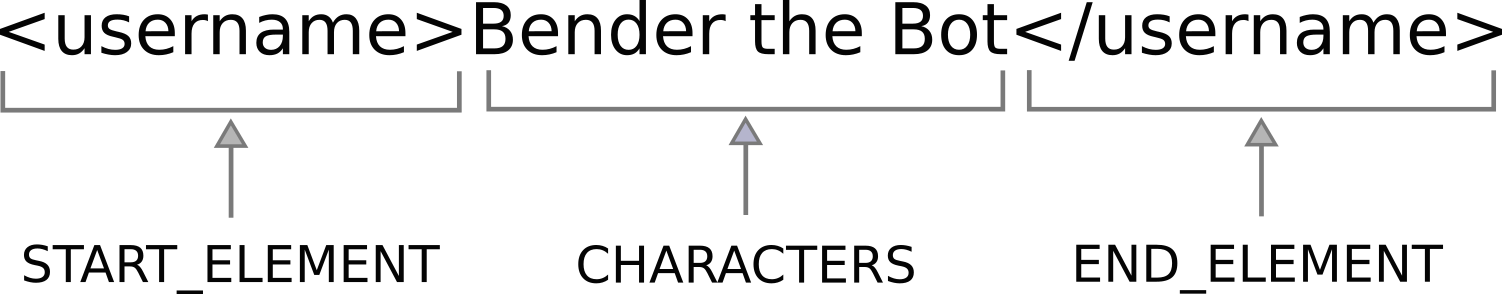
\includegraphics[width=0.6\textwidth]{image4}
	\caption{\small\sl Método {\tt\footnotesize getEventType}.}
	\captionsetup[figure]{list=yes}
\end{figure}

Assim sendo torna-se mais fácil trabalhar usando um conjunto de {\sl flags} demonstrado no excerto abaixo:

\begin{tcolorbox}[width=\textwidth,colback={darkgray},title={\sf Excerto 2.2: Como recolher o título do artigo.},outer arc=2mm,colupper=white]{\footnotesize\tt
		
	{\color{brightpink}case} {\color{lightblue}XMLStreamConstants}{\color{brightpink}.}{\color{newpink}START\_ELEMENT}{\color{brightpink}:}

    \tab {\color{lightblue}String} qName {\color{brightpink}=} reader{\color{brightpink}.}getLocalName();

	\tab {\color{brightpink}if}(qName{\color{brightpink}.}equalsIgnoreCase({\color{deadyellow}{"title}}\color{deadyellow}"\color{white}))\{
		
		\tab \tab bTitle {\color{brightpink}=} {\color{newpink}true};
	
	\tab \}
	{\color{brightpink}break};
	
	\tab \tab {\color{darkgray}...}
	
	{\color{brightpink}case} {\color{lightblue}XMLStreamConstants}{\color{brightpink}.}{\color{newpink}CHARACTERS}{\color{brightpink}:}
	
	\tab {\color{brightpink}if}(bTitle)\{
	
	\tab \tab title {\color{brightpink}=} reader{\color{brightpink}.}getText();
	
	\tab \tab bTitle {\color{brightpink}=} {\color{newpink}false};
	
	\tab \}
	{\color{brightpink}break};

}
\end{tcolorbox} 

Para toda a informação que quisermos retirar do XML temos de aplicar o que foi feito para o título do artigo no excerto acima. Então como vamos guardar a informação guardada quando chegamos ao fim de um artigo? 

O nosso método para resolver este problema foi criar uma {\tt writeFlag} para sinalizar quando devemos escrever numa estrutura a informação recolhida do XML. Essa {\tt writeFlag} é ativada quando recolhemos a última informação que desejamos do artigo, ou seja, após recolhermos o tamanho e palavras do texto.

Esta {\tt writeFlag} é imediatamente "desligada" quando chegamos ao fim da {\sl tag page} fazendo uso do evento {\tt END\_ELEMENT}.

\begin{tcolorbox}[width=\textwidth,colback={darkgray},title={\sf Excerto 2.3: Funcionamento da {\tt\footnotesize writeFlag}.},outer arc=2mm,colupper=white]{\footnotesize\tt
		
		{\color{brightpink}case} {\color{lightblue}XMLStreamConstants}{\color{brightpink}.}{\color{newpink}START\_ELEMENT}{\color{brightpink}:}
		
		\tab {\color{lightblue}String} qName {\color{brightpink}=} reader{\color{brightpink}.}getLocalName();
		
		\tab {\color{brightpink}if}(qName{\color{brightpink}.}equalsIgnoreCase({\color{deadyellow}{"text}}\color{deadyellow}"\color{white}))\{
		
		\tab \tab bTextSize {\color{brightpink}=} {\color{newpink}true};
	
		\tab \tab bTextWords {\color{brightpink}=} {\color{newpink}true};
		
		\tab \tab writeFlag {\color{brightpink}=} {\color{newpink}true};
		
		\tab \}
		{\color{brightpink}break};
		
		\tab \tab {\color{darkgray}...}
		
		{\color{brightpink}case} {\color{lightblue}XMLStreamConstants}{\color{brightpink}.}{\color{newpink}CHARACTERS}{\color{brightpink}:}
		
		\tab {\color{brightpink}if}(writeFlag)\{
		
		\tab \tab art {\color{brightpink}= new} {\color{lightblue}ArticleStructure}(title,id,revid,time,name,contid,
		
		\tab \tab \tab size,words);
		
		\tab \tab {\color{brightpink} return} art;
		
		\tab \}
		{\color{brightpink}break};
		
		\tab \tab {\color{darkgray}...}
		
		{\color{brightpink}case} {\color{lightblue}XMLStreamConstants}{\color{brightpink}.}{\color{newpink}END\_ELEMENT}{\color{brightpink}:}
				
   		\tab {\color{lightblue}String} qNames {\color{brightpink}=} reader{\color{brightpink}.}getLocalName();

		\tab {\color{brightpink}if}(qNames{\color{brightpink}.}equalsIgnoreCase({\color{deadyellow}{"text}}\color{deadyellow}"\color{white}))\{
		
		\tab \tab writeFlag {\color{brightpink}=} {\color{newpink}false};
		
		\tab \}
		{\color{brightpink}break};

	}
\end{tcolorbox} 








\section{Implementação da Estrutura}

Para guardar as informações relativas a um artigo criamos uma classe {\tt ArticleStructure}. Nela vamos guardar toda a informação que necessitamos relativamente a um artigo:


\begin{tcolorbox}[width=\textwidth,colback={darkgray},title={\sf Excerto 2.4: Classe {\tt\footnotesize ArticleStructure}.},outer arc=2mm,colupper=white]    
	{\footnotesize\ttfamily 
		
		{\color{brightpink}public class} {\color{lightblue}ArticleStructure}\{

		\tab {\color{brightpink}private} {\color{lightblue}String} title;
		
		\tab {\color{brightpink}private} {\color{lightblue}long} id;	
		
		\tab {\color{brightpink}private} {\color{lightblue}long} revid;
		
		\tab {\color{brightpink}private} {\color{lightblue}String} timestamp;
		
		\tab {\color{brightpink}private} {\color{lightblue}String} contributor;
		
		\tab {\color{brightpink}private} {\color{lightblue}long} contid;
		
		\tab {\color{brightpink}private} {\color{lightblue}long} size;
		
		\tab {\color{brightpink}private} {\color{lightblue}long} words;
		
		\tab {\color{gray}...}
		\
	}
\end{tcolorbox} 

Tal como foi feito no projeto em {\sl C} criamos também uma classe de contribuidores com menos informação (ID, ID da revisão, Contribuidor, ID do contribuidor) que vai servir para criar uma hashmap orientada pelos ID's dos contribuidores que vai ajudar na resolução de 2 questões.

Neste projeto voltamos a recorrer a uma tabela de hash para guardar as informações. Este método revela-se útil pois é muito mais fácil encontrar o que pretendemos quando temos a {\sl key} da hash onde procurar. Aqui, as tabelas de hash serão orientadas pelos ID's de artigo na hash de artigos e pelos ID's de contribuidor na hash de contribuidores.

\begin{tcolorbox}[width=\textwidth,colback={darkgray},title={\sf Excerto 2.5: Criar tabelas de hash.},outer arc=2mm,colupper=white]    
	{\footnotesize\ttfamily 
		
	artHash {\color{brightpink}= new} {\color{lightblue}HashMap<Long,ArrayList<ArticleStructure>>}();
	
	contHash {\color{brightpink}= new} {\color{lightblue}HashMap<Long,ArrayList<ContributorStructure>>}();
		\
	}
\end{tcolorbox} 

O ficheiro {\sl Load.} é o responsável pela leitura do XML e sua organização nas respetivas estruturas. Neste ficheiro temos uma função principal, a {\tt Load} que carrega os backups e que por cada artigo vai invocar a função {\tt buildArt} que lê o XML e cria as estruturas e a insere-as nas respetivas tabelas de hash através das respetivas funções de inserção ({\tt insertArt} e {\tt insertCont}).

\begin{figure}[h]
	\centering
	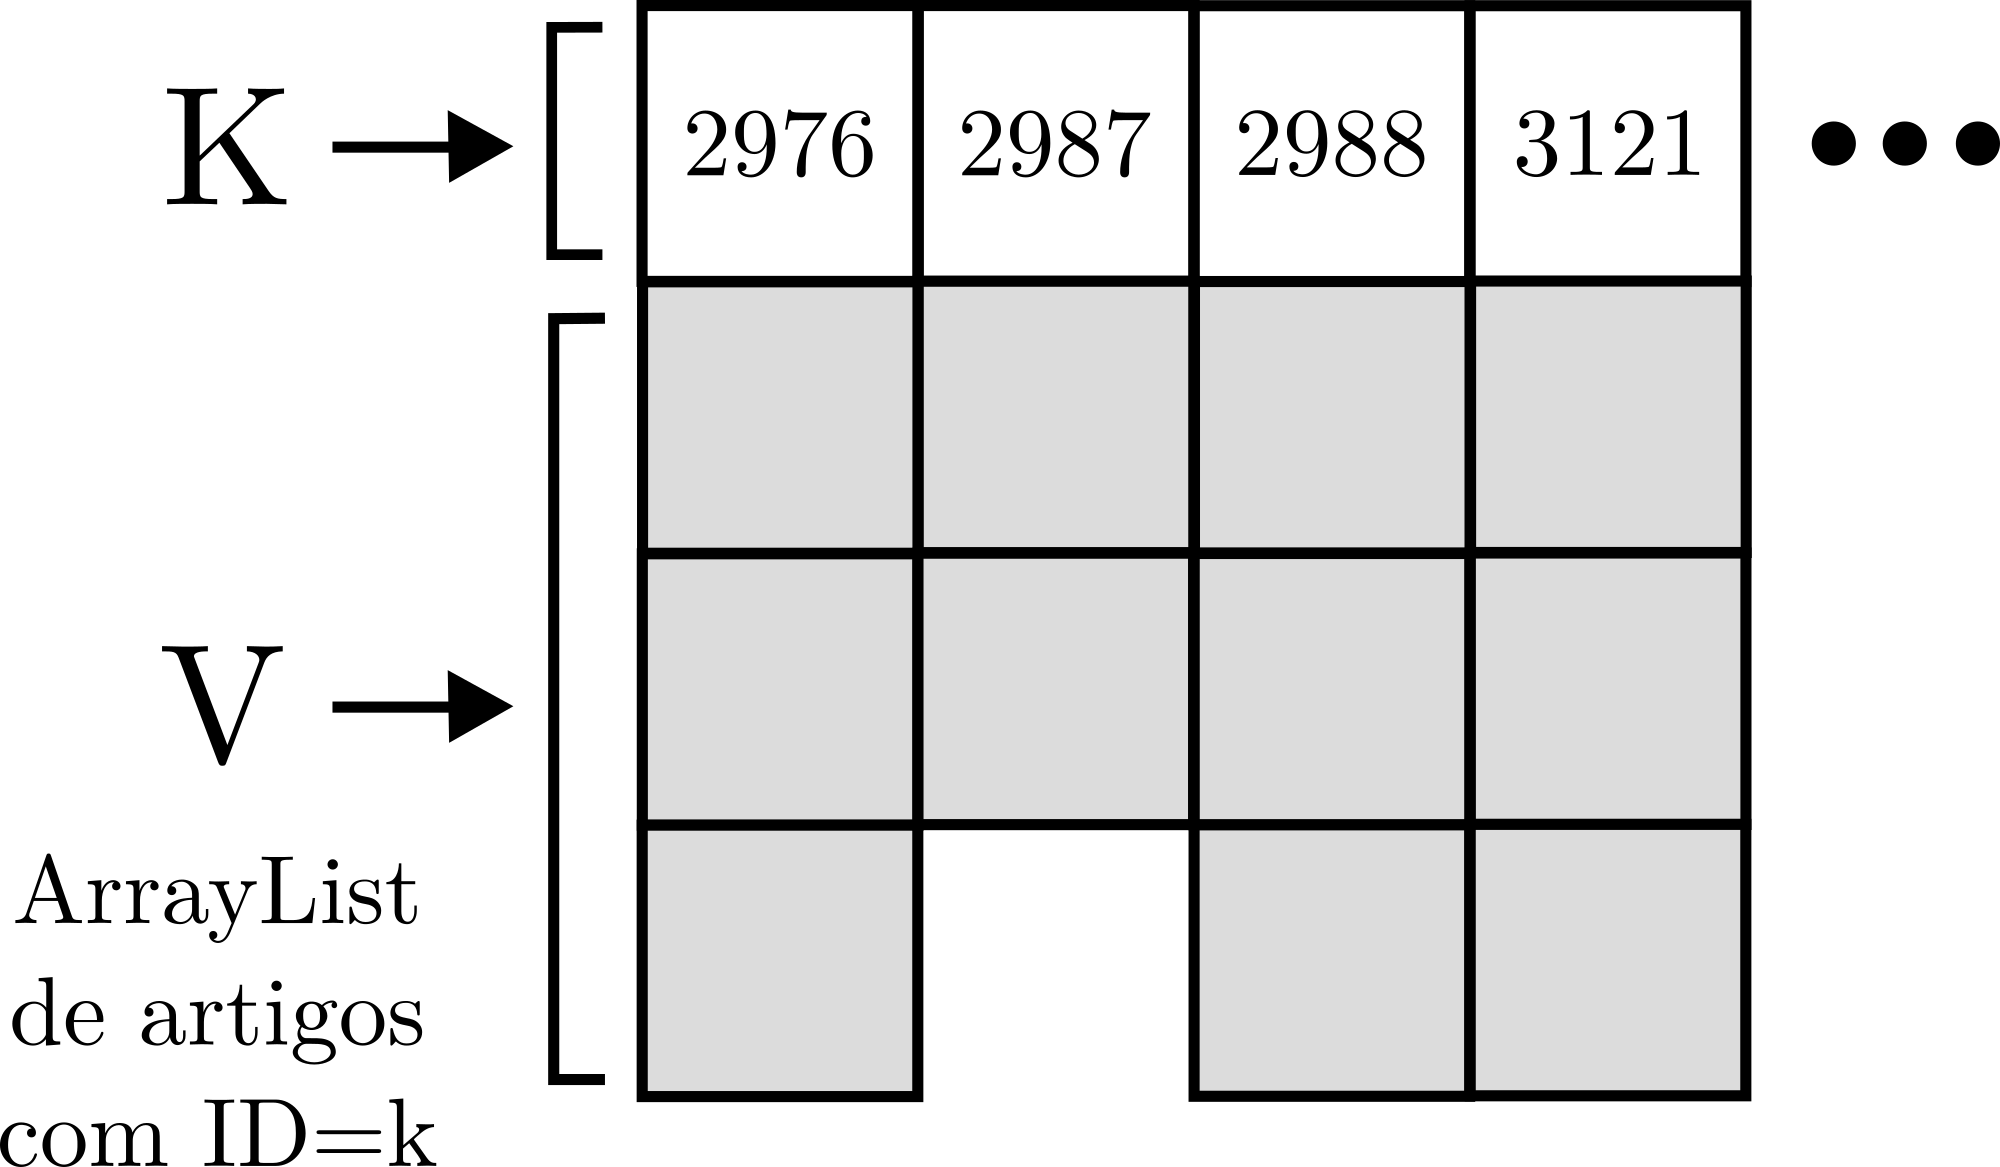
\includegraphics[width=0.5\textwidth]{image5}
	\caption{\small\sl Organização da hash dos artigos. A hash de contribuidores será igual, sendo que o {\sl K} será o ID do contribuidor}
	\captionsetup[figure]{list=yes}
\end{figure}

\section{Operações à Estrutura}

No ficheiro {\sl QueryEngineImpl.java} temos três funções para além das interrogações, a {\tt init}, {\tt load} e a {\tt clean}.

A {\tt init} tem a função de inicializar as duas tabelas de hash por omissão.

A {\tt load} carrega as tabelas de hash com a informação lida dos XML na classe {\tt Load}.

A {\tt clean} invoca o método {\tt clear()} da API de {\sl Hashmap} e limpa as estruturas de hash. Após esta função os mapas estarão vazios.

\section{Interrogações}

\begin{enumerate}
	\setlength\itemsep{0.00001em}
	\item A função {\tt\fontseries{b}\selectfont all\_articles} foi resolvida enquanto lemos os ficheiros XML. Como temos de saber sempre que um novo artigo começa para criar uma nova estrutura, criamos também uma variável que incrementa sempre que encontra um novo artigo e retornamos essa variável na função {all\_articles}.
	
	\item Para a {\tt\fontseries{b}\selectfont unique\_articles} como a hash tem como {\sl key} os ID's dos artigos e como {\sl value} um {\sl ArrayList} dos artigos desse ID, então o número de ID's únicos é o tamanho desta hash.

	\item Na {\tt\fontseries{b}\selectfont all\_revisions}, para cada {\sl key} (ID) vamos criar um {\sl ArrayList} com os ID's de revisão únicos daquele artigo. Quando chegarmos ao fim dos artigos daquele ID vamos adicionar o tamanho da lista criada, que será o números de revisões diferentes, a um contador. E passa para a próxima {\sl key}. No fim o contador deverá ter o número total de revisões diferentes.
	
	\item Para a {\tt\fontseries{b}\selectfont top\_10\_contributors} usamos a hash de contribuidores. Nesta hash criamos para cada contribuidor ({\sl key}) um {\sl Set} com os ID's de revisão únicos desse contribuidor e no fim dessa posição conta o tamanho do set e adiciona a um hashmap criado para a função, o ID do contribuidor como {\sl key} e o número de revisões únicas como {\sl value}. Após percorrer todas as posições da hash dos contribuidores iremos ter uma hash preenchida com todos os ID's de contribuidores e respetivo número de revisões. Usamos o pacote {\sl Java Stream} para ordenar pelo nº de revisões e cortar pelo tamanho 10. A {\sl key} da hash vai conter os ID's dos 10 maiores contribuidores, que será (e apenas a {\sl key}) copiada para um {\sl ArrayList}.
	
	\item Na {\tt\fontseries{b}\selectfont contributor\_name} fazemos proveitos das vantagens da hash. Uma vez que nos dão o ID do contribuidor basta ir para a {\sl key} igual a esse ID na hash dos contribuidores e obter o nome desse contribuidor num dos artigos desse contribuidor.
	
	\item A questão {\tt\fontseries{b}\selectfont top\_20\_largest\_articles} cria um hashmap onde irá guardar na {\sl key} o ID de artigo e no {\sl value} o tamanho desse artigo, caso não exista ou substituindo caso o tamanho seja maior do que o que já existia com aquele ID. Depois de completo o preenchimento do hashmap fazemos o mesmo {\sl stream} aplicado na {\tt top\_10\_contributors} e iremos ter um {\sl ArrayList} com os ID's ordenados pelos de maior tamanho.
	
	\item Para a {\tt\fontseries{b}\selectfont article\_title}, uma vez que nos é dado o ID do artigo que queremos, apenas temos de ir à {\sl key} exata da hashmap de artigos e devolver o título do artigo mais recente (que irá ser o último elemento do {\sl ArrayList} de artigos).
	
	\item Na função {\tt\fontseries{b}\selectfont top\_N\_articles\_with\_more\_words} usamos exatamente o mesmo método que na {\tt top\_20\_largest\_articles}, com a única diferença que o hashmap vai ser populado com o ID de artigo e respetivo número de palavras.
	
	\item Na questão {\tt\fontseries{b}\selectfont titles\_with\_prefix} percorremos cada posição da hash e em cada uma verificamos se o título dos artigos tem como prefixo a {\sl String} dada usando para isso a função predefinida em {\sl Java} {\tt startsWith()}. Se esta condição se verificar (ou seja, se a {\sl String} dada for, de facto, um prefixo do título) é adicionado o título a um {\sl ArrayList} e verificado se este não está já inserido. No fim o {\sl ArrayList} é ordenado alfabeticamente recorrendo a outra função predifinida, a {\tt sort()}.
	
	\item Para a última questão, a {\tt\fontseries{b}\selectfont article\_timestamp}, usamos o facto de nos ser dado o ID do artigo para ir imediatamente para a posição da hash onde este se encontra e a partir daí procuramos qual artigo coincidia com o ID de revisão e retornamos a {\sl timestamp} dessa revisão.
\end{enumerate}




\chapter {Conclusão}

Após concluirmos o trabalho as primeiras impressões que temos é que o tempo de execução é bem mais demorado do que o projeto anterior desenvolvido em {\sl C}. Verificamos que a maioria do tempo gasto é durante o processo de {\sl Load}, mais especificamente nas funções de contagem de palavras e de tamanho do texto.

Por outro lado a implementação das estruturas e a resolução das interrogações é muito mais fácil e rápida, ocupando muito menos linhas.

O pacote {\sl Java Stream} revelou-se bastante útil em algumas questões porque permite fazer em poucas linhas o que em {\sl C} iria implicar a criação de ciclos e outros.

No geral os nossos objetivos foram concluídos, sendo que todas as perguntas foram concluídas e aperfeiçoadas na medida do possível, tendo sempre em vista um código bem organizado e limpo.

\end{document}